\chapter{Data}\label{ch:style}
\section{TMK Dataset}

The TMK dataset was created by Goldsmith, Butcher, Benjamin, Sowmya, Muchlinski (2020) in  \emph{“Introducing The Targeted Mass Killing Dataset for the Study and Forecasting of Mass Atrocities”} \cite{Goldsmith2013}
The TMK dataset was created to contribute to the study into various atrocities such as genocide and politicide. 

The TMK dataset records events from 1946-2019 and tracks a wide variety of socioeconomic factors. The scale of the TMK event is quantified via a pre-coded ordinal indicator that aggregates evidence of intent as well as number of deaths. The scale and corresponding criteria for that classification is shown in Table 3.1. If time permits this project will try to produce a model that attempts to predict the severity of the TMK via the TMK ordinal indicator.
\begin{center}
\begin{table}
\begin{center}
 \begin{tabular}{||c c c||} 
 \hline
 Score & Intent & Total Deaths\\ [1ex] 
 \hline
 1 & NO Stated OR Organizational Intent & $25 \leq x \leq 999$ \\ [1ex] 
 \hline
 2 & NO Stated OR Organizational Intent &  $\geq 1000$  \\ [1ex] 
 \hline
 3 & Stated OR Organizational Intent & $25 \leq x \leq 999$ \\ [1ex]  
 \hline
  & TMK GENOCIDE/POLITICIDE THRESHOLD & \\
 \hline
 4 & Stated AND Organizational Intent  &  $\geq 1000$  \\ [1ex] 
 \hline
  5 & Stated AND Organizational Intent  & $25 \leq x \leq 999$  \\ [1ex] 
 \hline
  6 & Stated AND Organizational Intent  &  $\geq 1000$   \\ [1ex] 
 \hline
  7 & Stated AND Organizational Intent  &  $\geq 10,000$   \\ [1ex] 
 \hline
  8 & Stated AND Organizational Intent  &  $\geq 100,000$   \\ [1ex] 
 \hline
\end{tabular}
\caption{TMK Severity}
\end{center}
\end{table}
\end{center}
\pagebreak
\subsection{Generating Training Dataset}
The training dataset for my model will be generated using the following steps
\begin{enumerate}
  \item Merge selected variables from TMK events with some other datasets.
  \item Remove duplicated rows.
  \item Created lagged target variables because It takes time for some factors to take effect.
\end{enumerate}

The process of generating training datasets this way has been done before by others and produced a dataset with an imbalanced ratio $\rho = 26$ which translates to about 96\% non-tmk events. An imbalanced ratio of this magnitude is to be expected in this project's training dataset.

\section{Alternative Data Sources}
\subsection{Social Conflict Analysis Database}
The Social Conflicts Analysis Database(SCAD) includes protests, riots, strikes, inter-communal conflicts, government violence against civilians and other forms of social conflict not systematically tracked in other conflict datasets. SCAD currently includes information social conflicts from 1990-2017, covering all of Africa and now also Mexico, Central America, and the Caribbean.
\subsection{Uppsala Conflict Data Program}
The Uppsala Conflict Data Program (UCDP) is the world’s main provider of data on organized violence and the oldest ongoing data collection project for civil war, with a history of almost 40 years. Its definition of armed conflict has become the global standard of how conflicts are systematically defined and studied.
\subsection{Political Instability Task Force}
The Political Instability Task Force (PITF) is a U.S government project to construct a database on major domestic political conflicts leading up to state failures. Some variables that are tracked include the strength of a nations institutions and various social economic indicators such as infant mortality and life expectancy.
web-pages~\cite{Noo05}.
only.


\begin{figure}[h]
\centering
\includegraphics{data_compare.png}
\caption{Data Sources Comparison}
\end{figure}

A preliminary investigation of each other data sources has been conducted and it has been concluded that the SCAD database will be used in conjunction with the TMK dataset. This is mostly due to the high number of overlapping variables between the datasets. This makes merging the two via a full outer join easier as there will be less variables in the resultant dataset
\section{Data Issues}
\subsection{Class Imbalance}
As established in the literature review occurrences of TMKs are very rare and the generated training dataset is expected to have an imbalance ratio $\rho \approx  26$. There are a number of techniques that will be applied to resolve the class imbalance problem.

\subsubsection{Upsampling}
A common way of resolving the problem of class imbalance is upsampling where synthetic datapoints are artificially generated from the minority class

\begin{figure}[h]
\centering
\includegraphics{oversampling.png}
\caption{Upsampling}
\end{figure}

\subsubsection{Random Over-Sampling Examples(ROSE)}

The ROSE R package implements simple upsampling which involves populating empty features with zero-valued samples. ROSE also provides more robust upsampling where new datapoints are generated from the minority class based on the probability distribution and co-variance of the dataset. ROSE produces a \emph{"considerable amount of repeated observations amongst the rare examples"} ” (Lunardon, Menardi and Torelli, 2015, p84) \cite{Lunardo}. The ROSE algorithm is outlined in the figure below

\begin{figure}[h]
\centering
\includegraphics{rose_algo.png}
\caption{ROSE Algorithm}
\end{figure}

A weakness of ROSE is that if a large number of new data points are generated from a small subset of points it can lead to over fitting which will cause an increased generalization error (Fernandez et al, 2018, p83) \cite{Fernandez}. 

\subsubsection{Synthetic Minority Oversampling Technique(SMOTE)} 

\begin{figure}[h]
\centering
\includegraphics{knn.png}
\caption{SMOTE knn}
\end{figure}

Another technique for the generation of synthetic datapoints from the minority class is SMOTE. SMOTE randomly selects an instance from the minority class and applies the k nearest neighbours \cite{smotefamily}. A new datapoint is created by randomly selecting one the k nearest neighbours and connecting the two data points in the feature space. The new instance is generated as a convex combination of the two chosen instances. This allows new datapoints to be created based on topological properties in the neighborhood of the minority class, resulting in realistic datapoints. Figure 3.4 depicts how new datapoints are created in between the k nearest neighbours of the selected point.

\subsubsection{Downsampling}
An alternative to resolving the class imbalance problem without using upsampling is downsampling. Downsampling selects a subset of the majority class, this subset will be the same size as the minority class to ensure no class dominates the other. The selection of the subset is performed randomly.

\begin{figure}[h]
\centering
\includegraphics{downsampling.png}
\caption{Downsampling}
\end{figure}

The advantages of the downsampling is that it is very simple to perform and downsampling techniques are easily accessible via the R library ROSE. Additionally no overfitting will occur which is the case for upsampling techniques.

Disadvantages of downsampling are that potentially important information is lost from the datapoints of the majority class that are discarded, resulting in the model not being able to train on some features. Additionally if the class imbalance is very high there will only be a small pool of minority samples that are of greater interest to the model. Since the number of majority samples must be the same size as the ones from the minority class, the resultant dataset will be tiny and will not contain enough data for the model to train on


\subsubsection{Strategy for Resolving Class Imbalance}
This project will apply both ROSE, SMOTE and downsampling to resolve the class imbalance issue. As the literature states that a combination of techniques produces the most robust dataset.\emph{"The combination of SMOTE and under-sampling performs better than plain under-sampling"} \cite{Lunardo}.By using a combination of techniques the downsides of individual techniques such as over-fitting and lost of important information will be mitigated.

\subsection{Missing Values}
Like most datasets in social science a lot of TMK events have missing values across various features. Fig 3.6 depicts a sample of some of the features in the TMK dataset and the percentage of missing values across all the events. 

\begin{figure}[h]
\centering
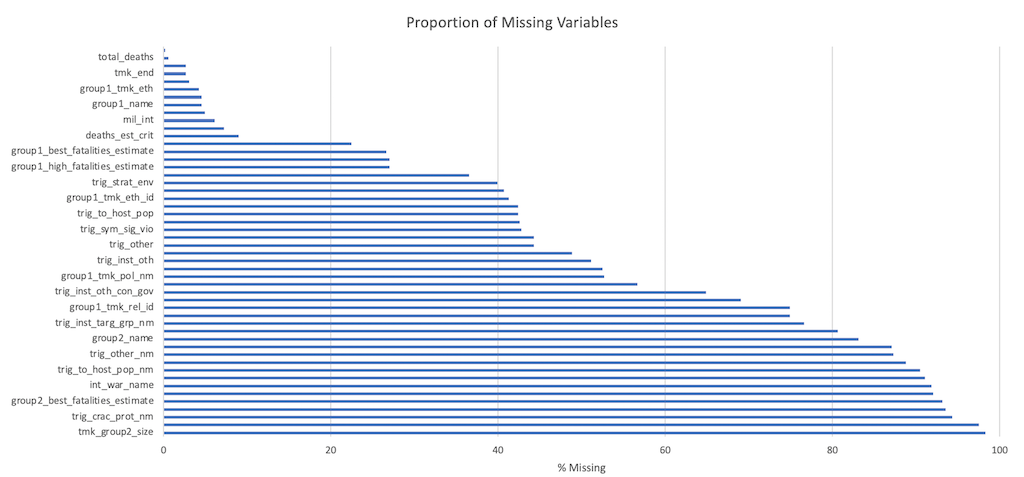
\includegraphics{proportionOfMissingvalues.png}
\caption{Proportion of missing values in TMK dataset}
\end{figure}


\subsubsection{Logical Imputations}
Logical imputation involves replacing missing values when the logic is obvious. For example, missing values can be logically imputated for TMK related because the dataset contains only TMK events.

\subsubsection{Multivariate Imputation Chained Equations}
Multivariate Imputation via Chained Equations (MICE) comprises of two techniques as outlined by Van Buren (2018) \cite{vanBuren}. The database contains missing values that match a \emph{"general pattern of missing data"}. 

MICE implements two methods for imputation of missing values. The first is Joint Modelling(JM) where imputations are drawn from a multivariate model fitted to data. The second is Fully Conditional Specification (FCS) involves drawing imputations from iterated conditional models. 

Both JM and FCS are available in R via the MICE package. A limitation of using the MICE package is that it can affect the bias and standard error of the data.

\begin{figure}[h]
\centering
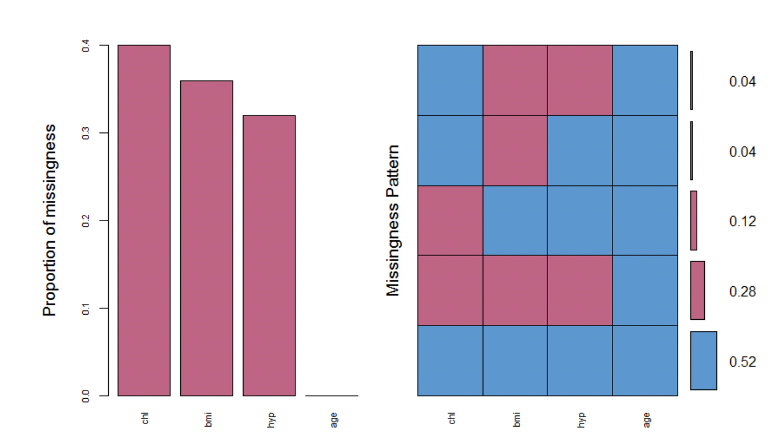
\includegraphics{missingdataimage.png}
\caption{General pattern of missing data visualized. Missing data in red}
\end{figure}


\subsection{Feature Explosion}
The TMK dataset already contains 121 different features. When additional datasets are merged via an outer join the number of features will only increase. When a model has to train on too many features it will encounter difficulty in identifying important features from less useful ones. This is known as the curse of dimensionality. 

To deal with the problem of feature explosion we will apply the Recursive Feature Elimination Algorithm(RFE) which is availability in the sklearn framework in python. 

As depicted in Fig 3.8 the RFE  algorithm recursively removes features at each step and re-ranks remaining features by retraining support vector machines based on these remaining features. If a feature is a weak feature, RFE will simply remove it. This apporach may present issues, because a weak feature may still be an important feature when used in conjunction with other features. 

\begin{figure}[h]
\centering
\includegraphics{rfe.png}
\caption{Recursive Feature Elimination Algorithm \cite{Furianello}}
\end{figure}
